%%%%%%%%%%%%%%%%%%%%%%%%%%%%%%%%%%%%%%%%%%%%%%%%%%%%%%%%%%%%%%%%%
\chapter{CHEST X-RAYS}
\label{ch:CH2}
%%%%%%%%%%%%%%%%%%%%%%%%%%%%%%%%%%%%%%%%%%%%%%%%%%%%%%%%%%%%%%%%%

X-rays (or X-radiations) are electromagnetic waves which is actually a type of radiation with wavelengths shorter than ultraviolet light. German physicist Wilhelm Konrad Röntgen discovered this specific type of energy photons while investigating cathode rays in Crookes tubes in 1895. Thereafter, Röntgen named this rays as X-rays to identify an unknown type of radiation. The first medical X-ray print can be found in Figure~\ref{fig:first_medical_xray}. 

On the other hand, a chest X-ray, or in other words a chest radiograph, is a projection radiograph of the chest used to diagnose health problems associated with the chest and its surroundings. The first use of X-rays for chest imaging dates back to 1896. Nowadays, X-rays are mostly used for medical and radiological imaging in medical industry and for security reasons in public areas.

The fewest photons are absorbed by the air, while the most photons are absorbed by the calcium in the bones. This is why bones appear white on X-ray images. Fat and other soft tissues moderately absorb X-rays, so they appear gray. Due to the aforementioned absorption properties of X-rays, the lungs appear blackish.

\begin{figure}[h]
    \centering
    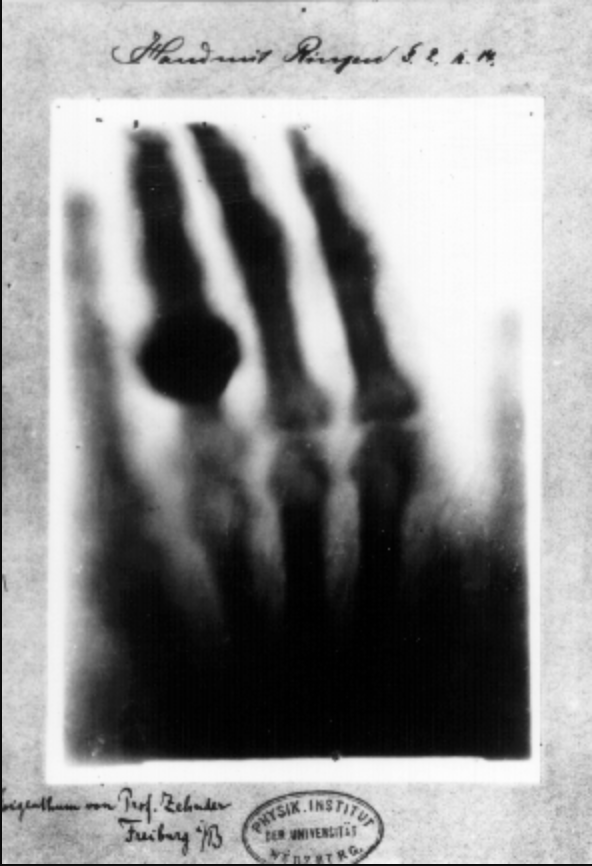
\includegraphics[keepaspectratio=true, scale=0.6]{./fig/first_medical_xray}
    % sekil2.eps: 0x0 pixel, 300dpi, 0.00x0.00 cm, bb=14 14 818 556
    \vspace*{3mm}
    \caption{Hand mit Ringen (Hand with Rings): the print of Wilhelm Röntgen's first medical X-ray of his wife's hand \cite{HandMitRingen}.}
    \label{fig:first_medical_xray}
\end{figure}

While the chest X-ray projection methods may vary from country to country or even from hospital to hospital, chest X-rays can be filmed through three main projection methods. The most preferred projection method is Posterior-Anterior (PA) view in which X-rays go through from patient's posterior to anterior. The patient has to be stand up during the operation. The second most used method is Anterior-Posterior (AP) erect view. On the contrary of frontal view, beams traverse from anterior to posterior in AP projection. When the PA or AP view is not possible due to the health issue of patient such that the patient may not able to stay erect, supine position is applied as AP-Supine projection method. The other most used view type is Lateral projection. It is performed from the left lateral of patient while the patient is standing. {An illustration of each projection method for chest X-rays for detecting COVID-19 is given in Figure~\ref{fig:chest_projections}. There are other various projection methods to film the chest of patient via X-rays.



\begin{figure}[h]
	\centering
	\subfigure[PA projection]{\label{fig:chest_projections_a}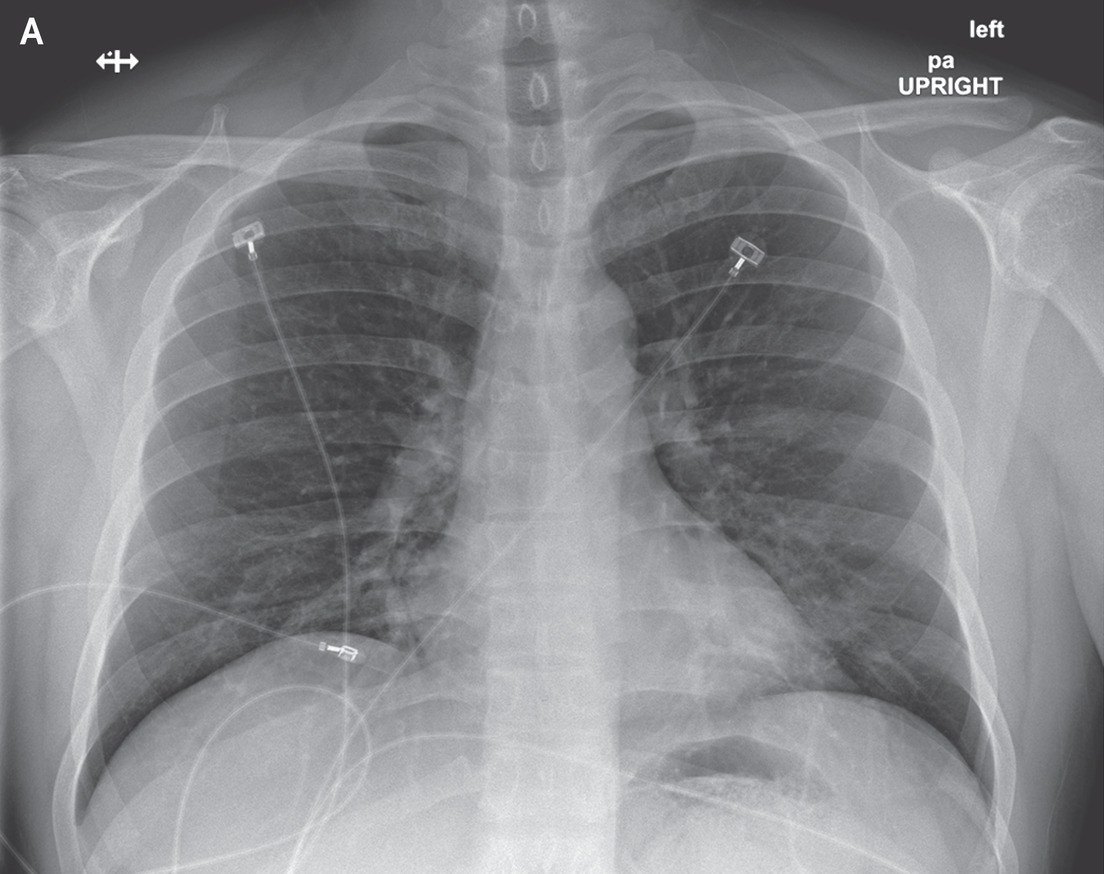
\includegraphics[width=.4\linewidth,height=.4\linewidth,scale=0.6]{chest_xray_PA}}
	\subfigure[AP projection]{\label{fig:chest_projections_b}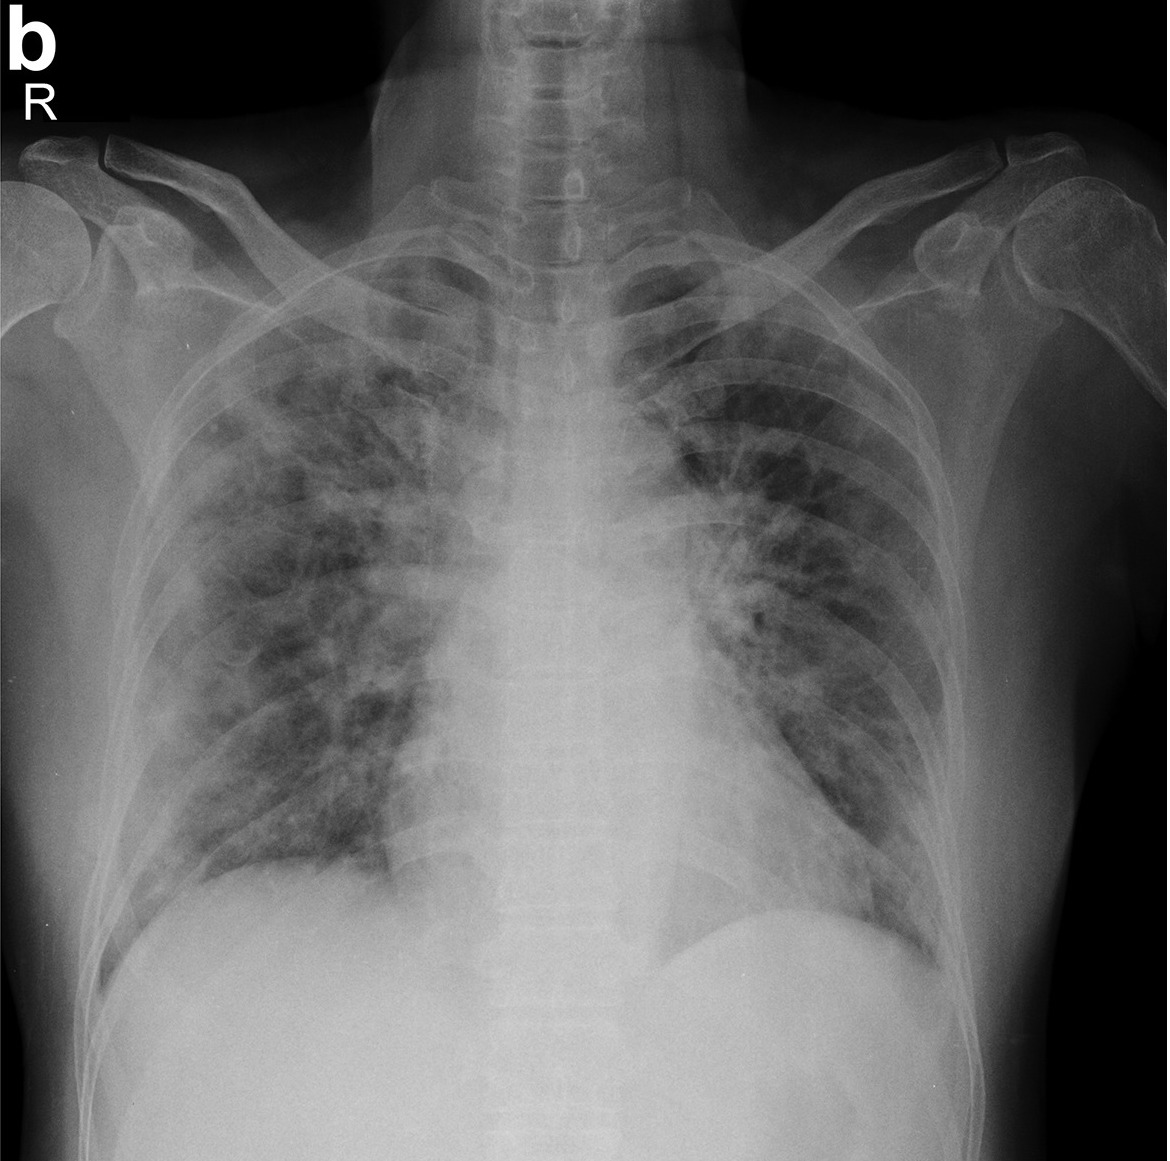
\includegraphics[width=.4\linewidth,height=.4\linewidth,scale=0.6]{chest_xray_AP}}
	\subfigure[AP-Supine projection]{\label{fig:chest_projections_c}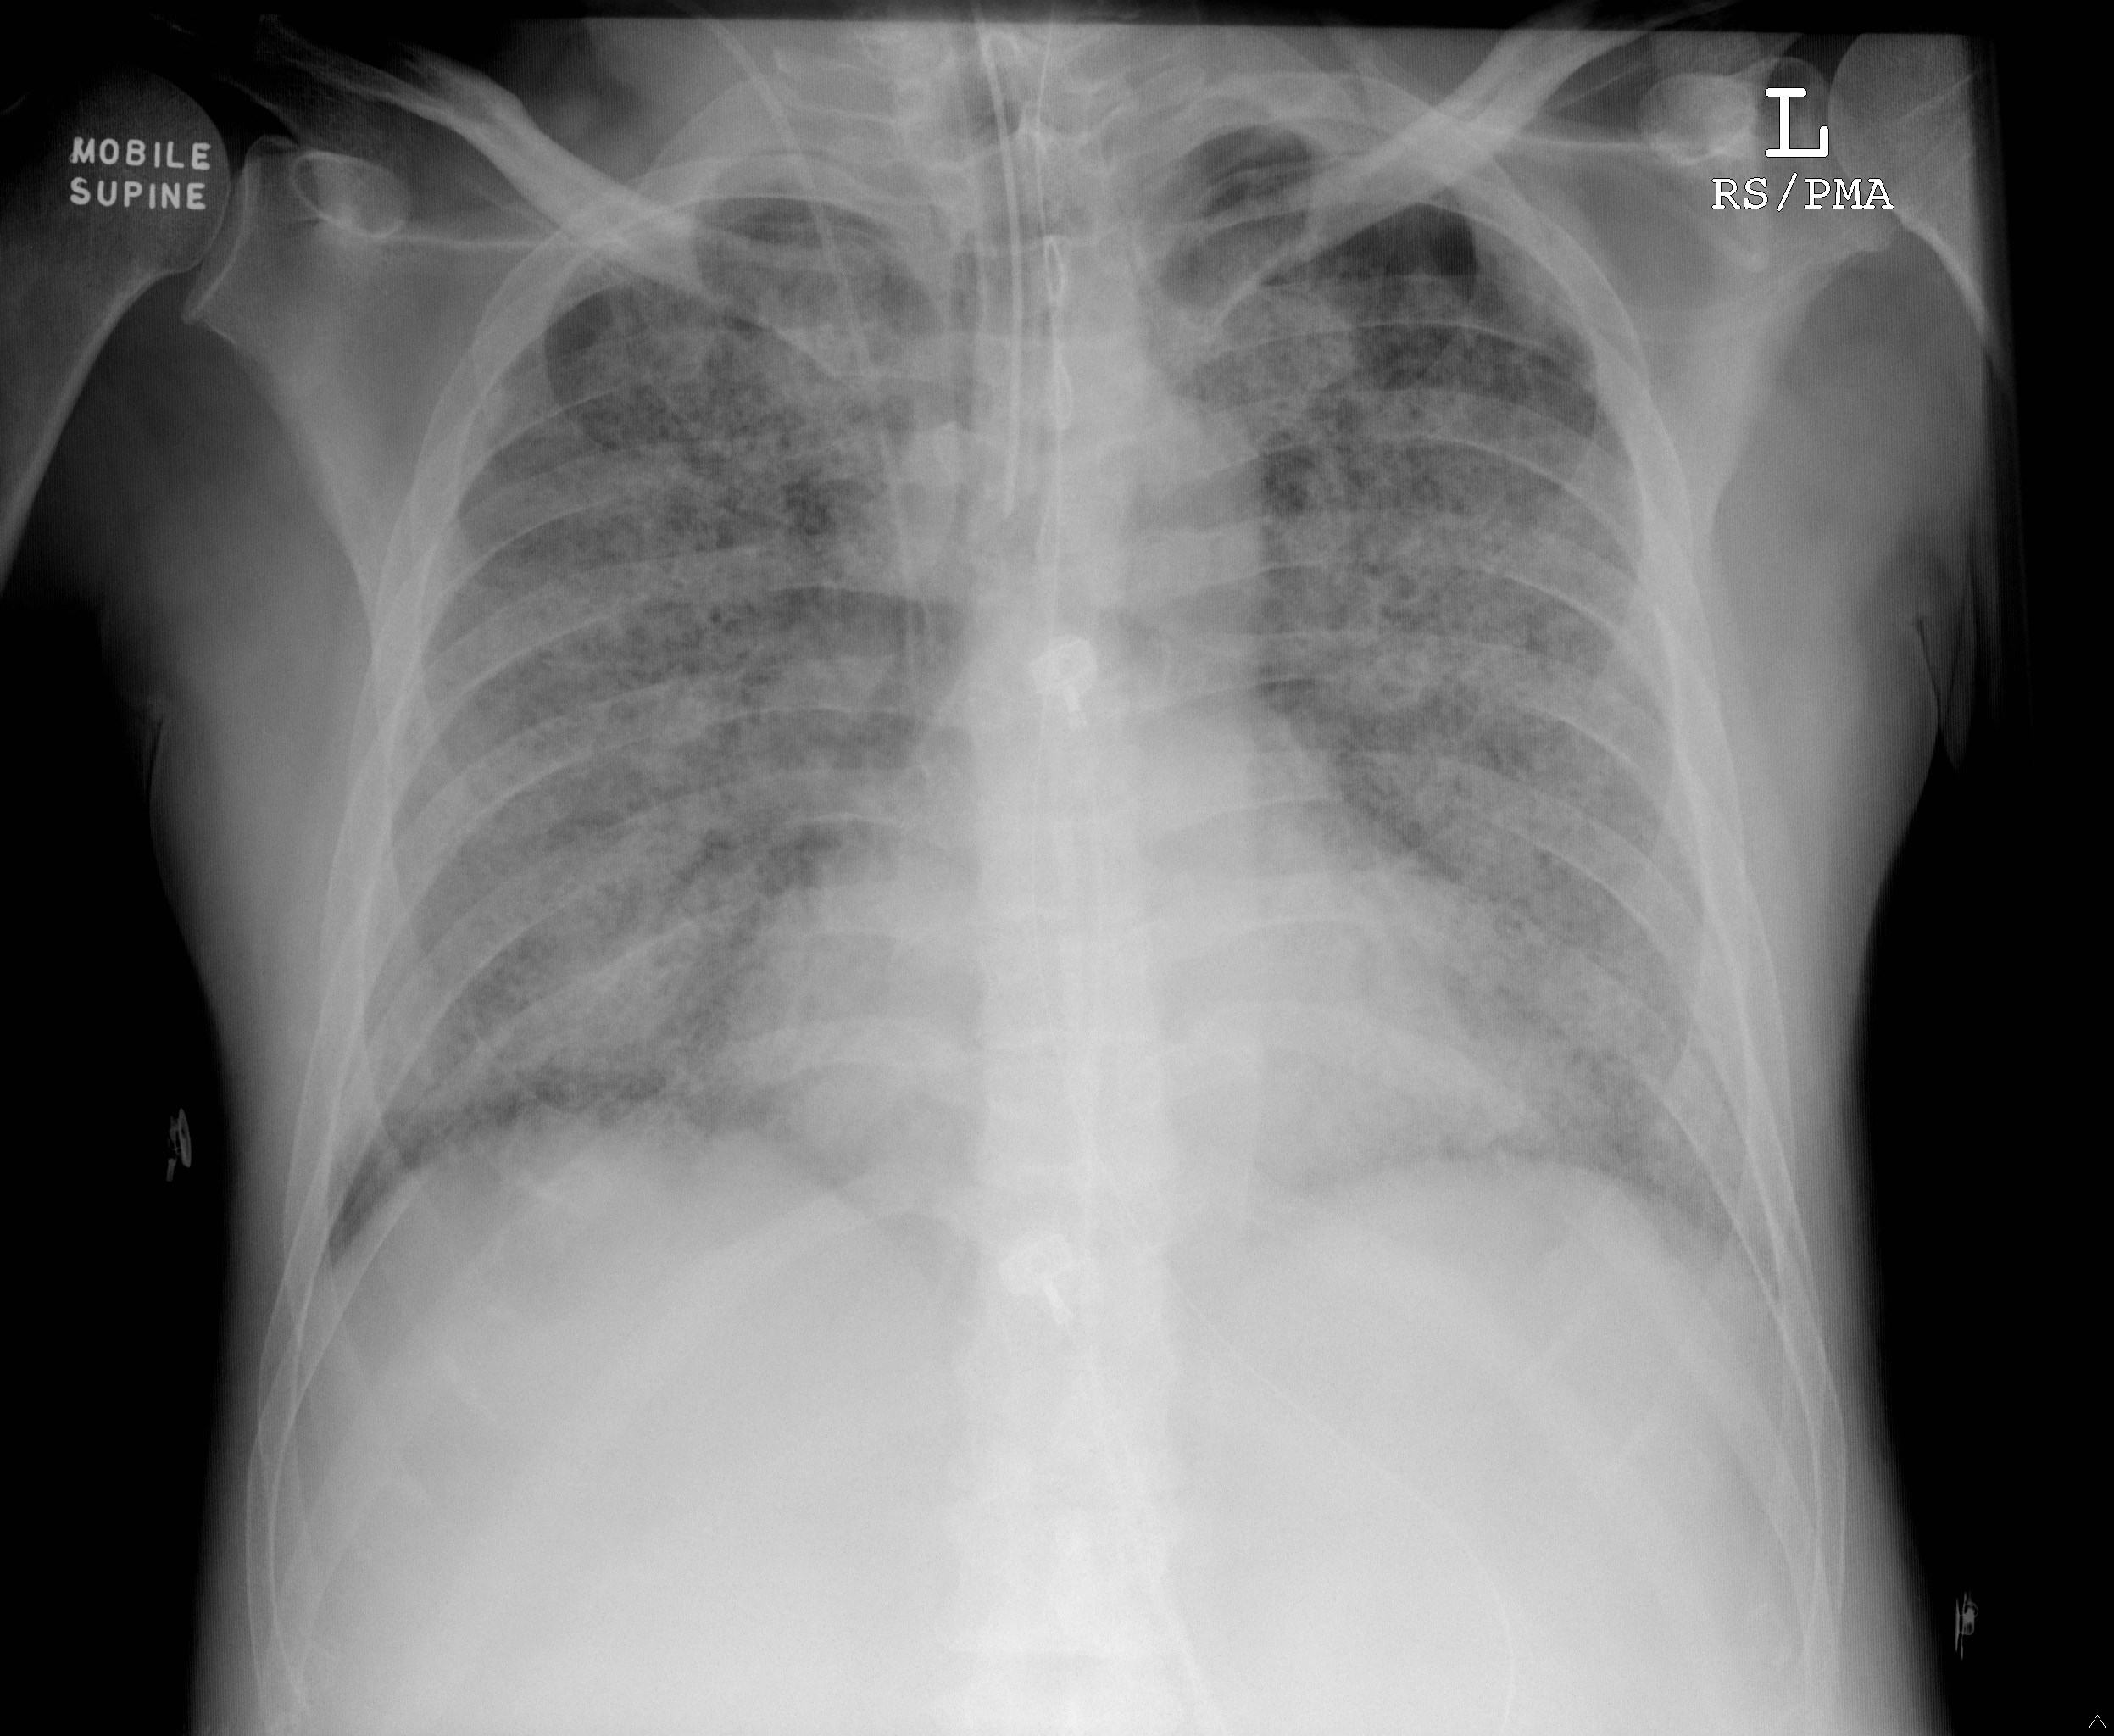
\includegraphics[width=.4\linewidth,height=.4\linewidth,scale=0.6]{chest_xray_AP_Supine}}
	\subfigure[L projection]{\label{fig:chest_projections_d}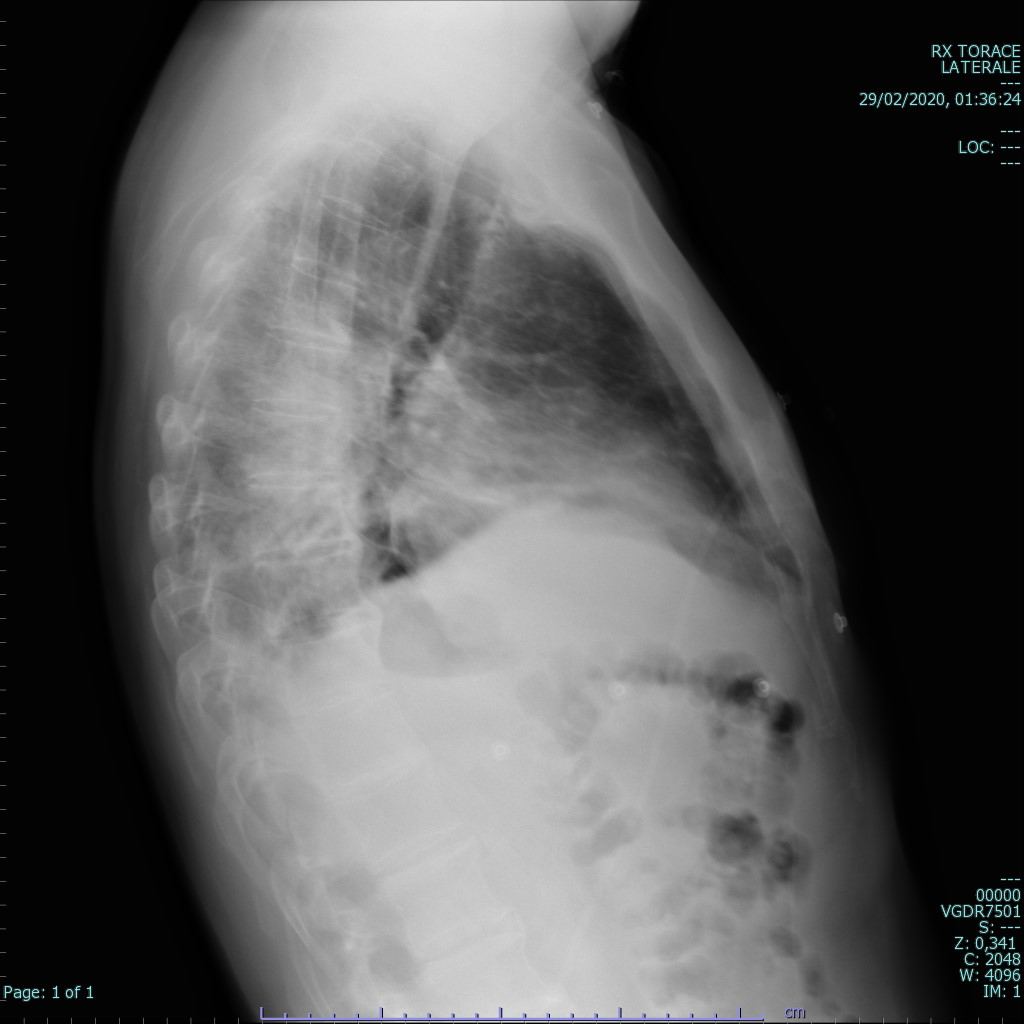
\includegraphics[width=.4\linewidth,height=.4\linewidth,scale=0.6]{chest_xray_L}}
	\captionfootnotemark{Examples for COVID-19 chest X-rays filmed with PA, AP, AP-Supine, and Lateral projections, respectively.}
	\label{fig:chest_projections}
\end{figure}
\footnotetext{Retrieved from GitHub: \hyperrefurl{https://github.com/ieee8023/covid-chestxray-dataset/tree/master/images} on March 25, 2021.}

Chest X-ray imaging has a very significant role on detecting serious diseases such as pneumonia and its causes, pneumothorax, heart failures, emphysema, lung cancer, broken ribs for years, and COVID-19 recently. Thanks to the accessibility and the ease of use of chest X-rays, various artificial intelligence problems can be formed and accomplished for the benefit of medical use, computer science, and mathematics.